\documentclass[xcolor=dvipsnames,serif]{beamer}\usepackage[]{graphicx}\usepackage[]{color}
%% maxwidth is the original width if it is less than linewidth
%% otherwise use linewidth (to make sure the graphics do not exceed the margin)
\makeatletter
\def\maxwidth{ %
  \ifdim\Gin@nat@width>\linewidth
    \linewidth
  \else
    \Gin@nat@width
  \fi
}
\makeatother

\definecolor{fgcolor}{rgb}{0.345, 0.345, 0.345}
\newcommand{\hlnum}[1]{\textcolor[rgb]{0.686,0.059,0.569}{#1}}%
\newcommand{\hlstr}[1]{\textcolor[rgb]{0.192,0.494,0.8}{#1}}%
\newcommand{\hlcom}[1]{\textcolor[rgb]{0.678,0.584,0.686}{\textit{#1}}}%
\newcommand{\hlopt}[1]{\textcolor[rgb]{0,0,0}{#1}}%
\newcommand{\hlstd}[1]{\textcolor[rgb]{0.345,0.345,0.345}{#1}}%
\newcommand{\hlkwa}[1]{\textcolor[rgb]{0.161,0.373,0.58}{\textbf{#1}}}%
\newcommand{\hlkwb}[1]{\textcolor[rgb]{0.69,0.353,0.396}{#1}}%
\newcommand{\hlkwc}[1]{\textcolor[rgb]{0.333,0.667,0.333}{#1}}%
\newcommand{\hlkwd}[1]{\textcolor[rgb]{0.737,0.353,0.396}{\textbf{#1}}}%
\let\hlipl\hlkwb

\usepackage{framed}
\makeatletter
\newenvironment{kframe}{%
 \def\at@end@of@kframe{}%
 \ifinner\ifhmode%
  \def\at@end@of@kframe{\end{minipage}}%
  \begin{minipage}{\columnwidth}%
 \fi\fi%
 \def\FrameCommand##1{\hskip\@totalleftmargin \hskip-\fboxsep
 \colorbox{shadecolor}{##1}\hskip-\fboxsep
     % There is no \\@totalrightmargin, so:
     \hskip-\linewidth \hskip-\@totalleftmargin \hskip\columnwidth}%
 \MakeFramed {\advance\hsize-\width
   \@totalleftmargin\z@ \linewidth\hsize
   \@setminipage}}%
 {\par\unskip\endMakeFramed%
 \at@end@of@kframe}
\makeatother

\definecolor{shadecolor}{rgb}{.97, .97, .97}
\definecolor{messagecolor}{rgb}{0, 0, 0}
\definecolor{warningcolor}{rgb}{1, 0, 1}
\definecolor{errorcolor}{rgb}{1, 0, 0}
\newenvironment{knitrout}{}{} % an empty environment to be redefined in TeX

\usepackage{alltt}
\usetheme{Boadilla}
\usecolortheme[named=CornflowerBlue]{structure}
\usepackage{graphicx}
\usepackage{breqn}
\usepackage{xcolor}
\usepackage{booktabs}
\usepackage{verbatim}
\usepackage{tikz}
\usepackage[final]{animate}
\usepackage{lmodern}
\usetikzlibrary{shadows,arrows,positioning}
\definecolor{links}{HTML}{2A1B81}
\hypersetup{colorlinks,linkcolor=links,urlcolor=links}
\usepackage{pgfpages}

\tikzstyle{block} = [rectangle, draw, text width=9em, text centered, rounded corners, minimum height=3em, minimum width=7em, top color = white, bottom color=brown!30,  drop shadow]

% change font of frame titles and title slide
\setbeamerfont{title}{series=\bfseries}
\setbeamerfont{frametitle}{series=\bfseries} 

% enumerate style
\setbeamertemplate{enumerate items}[circle]

% my macros
\newcommand{\ShowSexpr}[1]{\texttt{{\char`\\}Sexpr\{#1\}}}
\newcommand{\Bigtxt}[1]{\textbf{\textit{#1}}}
\IfFileExists{upquote.sty}{\usepackage{upquote}}{}
\begin{document}

\title[Seasonal Kendall]{Time series topic 3: Seasonal Kendall Tests}

\author[M. Beck]{Marcus W. Beck\inst{1}}

\date{}

\institute[]{\inst{1} USEPA NHEERL Gulf Ecology Division\\ Email: \href{mailto:beck.marcus@epa.gov}{beck.marcus@epa.gov}}

% knitr setup


% dependents


% get online bib file


%%%%%%
\begin{frame}
\vspace{0.3in}
\centerline{
\begin{tikzpicture}
  \node[drop shadow={shadow xshift=0ex,shadow yshift=0ex},fill=white,draw] at (0,0) {
\includegraphics[width=0.9\textwidth]{imgs/workshop2016logo.png}};
\end{tikzpicture}}
\titlepage
\end{frame}

\section{Overview}

%%%%%%
\begin{frame}{Objectives for the session (4:15 - 5:00)}{}
\begin{itemize}
\item What is and why would we use a Kendall test \\~\\
\item What is a why would we use a \textit{Seasonal} Kendall test \\~\\
\item Application with NERRS data \\~\\
\begin{itemize}
\item Data prep \\~\\
\item Execution \\~\\
\item Interpretation
\end{itemize}
\end{itemize}
\end{frame}

%%%%%%
\begin{frame}{Interactive portion}
\onslide<+->
Follow along as we go:\\~\\
\begin{itemize}
\item flash drive\\~\\
\item online: \href{http://swmprats.net/}{swmprats.net} 2016 workshop tab \\~\\
\end{itemize}
\onslide<+->
You will run examples whenever you see this guy: \\~\\
\centerline{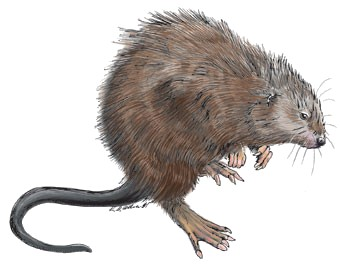
\includegraphics[width = 0.15\textwidth]{imgs/swmprat.png}}
\end{frame}

%%%%%%
\begin{frame}[fragile]{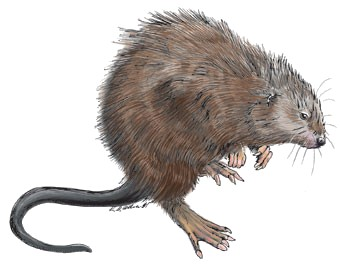
\includegraphics[width = 0.05\textwidth]{imgs/swmprat.png} Is everything installed?}
\onslide<1->
We will use functions in the EnvStats package \\~\\
Option 1, from the R Console prompt:
\begin{knitrout}\scriptsize
\definecolor{shadecolor}{rgb}{0.969, 0.969, 0.969}\color{fgcolor}\begin{kframe}
\begin{alltt}
\hlkwd{install.packages}\hlstd{(}\hlstr{'EnvStats'}\hlstd{)}
\hlkwd{library}\hlstd{(EnvStats)}
\end{alltt}
\end{kframe}
\end{knitrout}
\onslide<2->
\vspace{0.1in}
Option 2, install the source file from the flash drive:
\begin{knitrout}\scriptsize
\definecolor{shadecolor}{rgb}{0.969, 0.969, 0.969}\color{fgcolor}\begin{kframe}
\begin{alltt}
\hlcom{# change as needed}
\hlstd{path_to_file} \hlkwb{<-} \hlstr{'C:/Users/mbeck/Desktop/EnvStats_2.1.1.tar.gz'}

\hlcom{# install, load}
\hlkwd{install.packages}\hlstd{(path_to_file,} \hlkwc{repos} \hlstd{=} \hlkwa{NULL}\hlstd{,} \hlkwc{type}\hlstd{=}\hlstr{"source"}\hlstd{)}
\hlkwd{library}\hlstd{(EnvStats)}
\end{alltt}
\end{kframe}
\end{knitrout}
\end{frame}

%%%%%%
\begin{frame}[fragile]{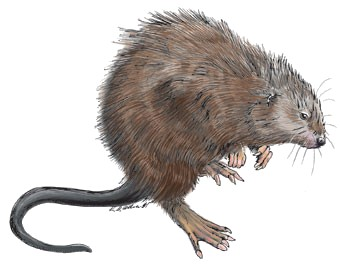
\includegraphics[width = 0.05\textwidth]{imgs/swmprat.png} Is everything installed?}
\onslide<1->
We will use functions in the lubridate package \\~\\
Option 1, from the R Console prompt:
\begin{knitrout}\scriptsize
\definecolor{shadecolor}{rgb}{0.969, 0.969, 0.969}\color{fgcolor}\begin{kframe}
\begin{alltt}
\hlkwd{install.packages}\hlstd{(}\hlstr{'lubridate'}\hlstd{)}
\hlkwd{library}\hlstd{(lubridate)}
\end{alltt}
\end{kframe}
\end{knitrout}
\onslide<2->
\vspace{0.1in}
Option 2, install the source file from the flash drive:
\begin{knitrout}\scriptsize
\definecolor{shadecolor}{rgb}{0.969, 0.969, 0.969}\color{fgcolor}\begin{kframe}
\begin{alltt}
\hlcom{# change as needed}
\hlstd{path_to_file} \hlkwb{<-} \hlstr{'C:/Users/mbeck/Desktop/lubridate_1.6.0.tar.gz'}

\hlcom{# install, load}
\hlkwd{install.packages}\hlstd{(path_to_file,} \hlkwc{repos} \hlstd{=} \hlkwa{NULL}\hlstd{,} \hlkwc{type}\hlstd{=}\hlstr{"source"}\hlstd{)}
\hlkwd{library}\hlstd{(lubridate)}
\end{alltt}
\end{kframe}
\end{knitrout}
\end{frame}

%%%%%%
\begin{frame}[t]{Theory and background}{}
\onslide<1->
Use these tests to answer the question: \\~\\
Is there a \Bigtxt{monotonic trend} and what is the \Bigtxt{significance}? \\~\\
\onslide<2->
Both tests:
\vspace{0.1in}
\begin{itemize}
\item Are non-parametric (no distribution assumptions, based on signs) \\~\\
\item<3-> Work with a user-defined time interval \\~\\
\item<4-> Provide a p-value indicating the probability due to chance alone \\~\\
\item<5-> Provide a direction of the trend as $\tau$ (`tau') \\~\\
\item<6-> Provide a slope as the rate of change
\end{itemize}
\end{frame}

%%%%%%
\begin{frame}[t]{Theory and background}{}
\onslide<1->
The \Bigtxt{Kendall test} for time series:
$$S = \sum_{i = 1}^{n - 1}\sum_{j = i + 1}^{n} sign\left[\left(X_j - X_i\right)\left(Y_j - Y_i\right)\right]$$
$$\hat{\tau} = \frac{2S}{n\left(n - 1\right)}$$
\begin{center}
$\hat{\tau}$ will vary from -1 to 1 similar to a correlation coefficient, follows an approximate normal-distribution for hypothesis-testing
\end{center}
\end{frame}

%%%%%%
\begin{frame}[t]{Theory and background}{}
\onslide<1->
The \Bigtxt{Kendall test} for time series:
$$\hat{\beta}_1 = Median\left(\frac{Y_j - Y_i}{X_j - X_i}\right), i < j$$
\begin{center}
$\hat{\beta}_1$ is the Theil (Sen) non-parametric estimate of slope or the rate of change in the interval
\end{center}
\onslide<2->
All you need to know:\\~\\
\begin{itemize}
\item $\hat{\tau}$ is direction and magnitude of trend \\~\\
\item $\hat{\beta}_1$ is the linear rate of change
\end{itemize}
\end{frame}

%%%%%%
\begin{frame}{Theory and background}{}
\onslide<1->
The \Bigtxt{Seasonal Kendall test} is exactly the same... \\
...except separate tests by month across years (January 1981, 1982, ..., February 1981, 1982, ...), results are pooled. \\~\\
\begin{itemize}
\item<2-> Overall $\hat{\tau}$ is the weighted average of the seasonal estimates \\~\\
\item<3-> Overall $\hat{\beta_1}$ is the median of all two-point slope estimates within each season \\~\\
\end{itemize}
\onslide<4->
More info in help documentation for \texttt{kendallTrendTest}, \texttt{kendallSeasonalTrendTest} in EnvStats, \cite{Hirsch82,Millard13}
\end{frame}

\section{Application}

%%%%%%
\begin{frame}{Using \texttt{kendallTrendTest} with NERRS data}{}
\includegraphics<1>[width = \textwidth]{imgs/noc_widg1.PNG}

\includegraphics<2>[width = \textwidth]{imgs/noc_widg2.PNG}
\end{frame}

%%%%%%
\begin{frame}{Using \texttt{kendallTrendTest} with NERRS data}{}
\onslide<1-> 
Using nutrient data from North Carolina NERR, Zeke's Basin site: \\~\\
\begin{enumerate}
\item<1-> Import nutrient data, prep\\~\\
\item<2-> Test with \texttt{kendallTrendTest}\\~\\
\item<3-> Interpret results
\end{enumerate}
\end{frame}

%%%%%%
\begin{frame}[fragile]{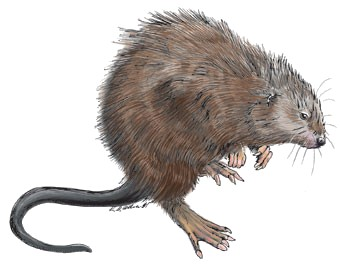
\includegraphics[width = 0.05\textwidth]{imgs/swmprat.png} Using \texttt{kendallTrendTest} with NERRS data}
\begin{enumerate}
\item<1-> Import nutrient data, prep
\end{enumerate}
\onslide<2->
\begin{knitrout}\scriptsize
\definecolor{shadecolor}{rgb}{0.969, 0.969, 0.969}\color{fgcolor}\begin{kframe}
\begin{alltt}
\hlcom{# load SWMPr, nutrient data}
\hlkwd{library}\hlstd{(SWMPr)}
\hlkwd{load}\hlstd{(}\hlkwc{file} \hlstd{=} \hlstr{'data/noczbnut.RData'}\hlstd{)}

\hlcom{# rename, qaqc clean up, subset}
\hlstd{nut} \hlkwb{<-} \hlstd{noczbnut}
\hlstd{nut} \hlkwb{<-} \hlkwd{qaqc}\hlstd{(nut,} \hlkwc{qaqc_keep} \hlstd{=} \hlkwd{c}\hlstd{(}\hlnum{0}\hlstd{,} \hlnum{4}\hlstd{))}
\hlstd{nut} \hlkwb{<-} \hlkwd{subset}\hlstd{(nut,} \hlkwc{select} \hlstd{=} \hlstr{'chla_n'}\hlstd{)}
\hlstd{nut} \hlkwb{<-} \hlkwd{na.omit}\hlstd{(nut)}
\hlkwd{head}\hlstd{(nut)}
\end{alltt}
\begin{verbatim}
##         datetimestamp chla_n
## 1 2002-04-23 15:35:00   2.12
## 2 2002-05-24 09:20:00   1.60
## 3 2002-06-24 10:35:00   3.47
## 4 2002-07-24 09:40:00   4.43
## 5 2002-08-26 11:31:00   4.65
## 6 2002-09-24 10:40:00   5.95
\end{verbatim}
\end{kframe}
\end{knitrout}
\end{frame}

%%%%%%
\begin{frame}[fragile, t]{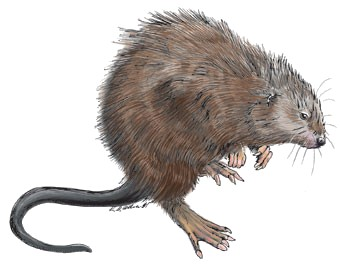
\includegraphics[width = 0.05\textwidth]{imgs/swmprat.png} Using \texttt{kendallTrendTest} with NERRS data}
\begin{enumerate}
\item<1-> Import nutrient data, prep
\end{enumerate}
First look at a plot:
\begin{knitrout}\scriptsize
\definecolor{shadecolor}{rgb}{0.969, 0.969, 0.969}\color{fgcolor}\begin{kframe}
\begin{alltt}
\hlkwd{plot}\hlstd{(nut)}
\end{alltt}
\end{kframe}

{\centering 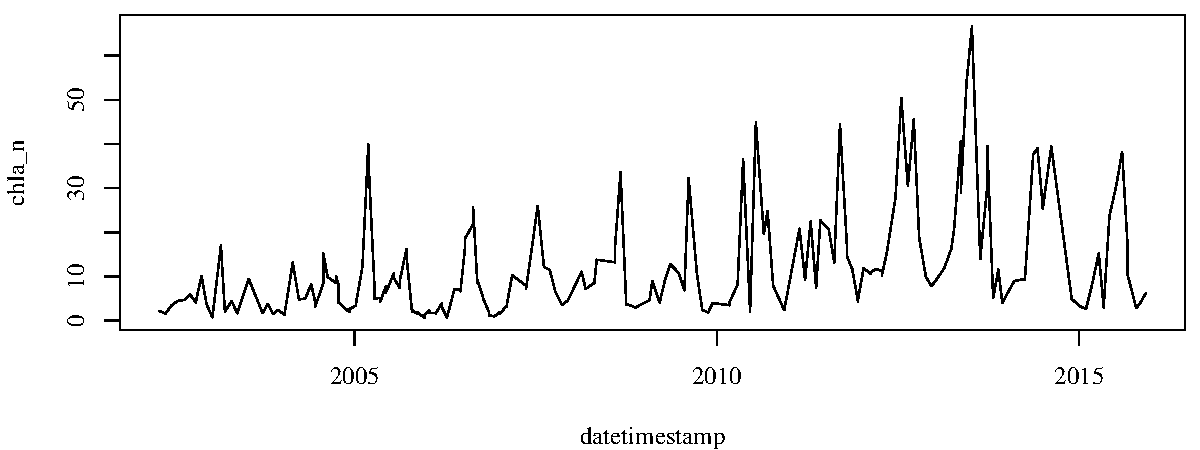
\includegraphics[width=\textwidth]{imgs/unnamed-chunk-7-1} 

}



\end{knitrout}
\end{frame}

%%%%%%
\begin{frame}[fragile, t]{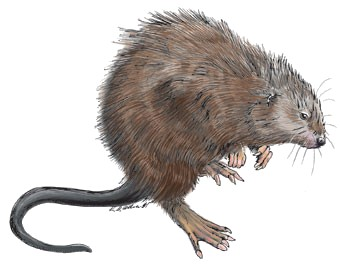
\includegraphics[width = 0.05\textwidth]{imgs/swmprat.png} Using \texttt{kendallTrendTest} with NERRS data}
\begin{enumerate}
\setcounter{enumi}{1}
\item Test with \texttt{kendallTrendTest}
\end{enumerate}
Run the test:
\begin{knitrout}\scriptsize
\definecolor{shadecolor}{rgb}{0.969, 0.969, 0.969}\color{fgcolor}\begin{kframe}
\begin{alltt}
\hlcom{# load libraries, add decimal date}
\hlkwd{library}\hlstd{(EnvStats)}
\hlkwd{library}\hlstd{(lubridate)}
\hlstd{nut}\hlopt{$}\hlstd{dec_yr} \hlkwb{<-} \hlkwd{decimal_date}\hlstd{(nut}\hlopt{$}\hlstd{datetimestamp)}

\hlcom{# run test}
\hlstd{ests_k1} \hlkwb{<-} \hlkwd{kendallTrendTest}\hlstd{(chla_n} \hlopt{~} \hlstd{dec_yr, nut)}
\hlstd{ests_k1}\hlopt{$}\hlstd{estimate}
\end{alltt}
\begin{verbatim}
##           tau         slope     intercept 
##     0.3146341     0.8865779 -1772.6181270
\end{verbatim}
\begin{alltt}
\hlstd{ests_k1}\hlopt{$}\hlstd{p.value}
\end{alltt}
\begin{verbatim}
##            z 
## 2.097253e-11
\end{verbatim}
\end{kframe}
\end{knitrout}
\end{frame}

%%%%%%
\begin{frame}[fragile, t]{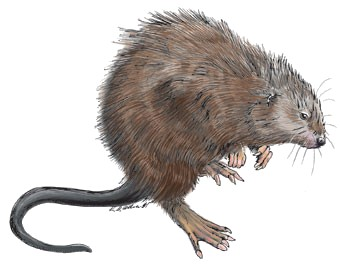
\includegraphics[width = 0.05\textwidth]{imgs/swmprat.png} Using \texttt{kendallTrendTest} with NERRS data}
\begin{enumerate}
\setcounter{enumi}{2}
\item Interpret results
\end{enumerate}
Do they make sense? Check seasonality in observed data:
\begin{knitrout}\scriptsize
\definecolor{shadecolor}{rgb}{0.969, 0.969, 0.969}\color{fgcolor}\begin{kframe}
\begin{alltt}
\hlkwd{plot_summary}\hlstd{(nut,} \hlkwc{param} \hlstd{=} \hlstr{'chla_n'}\hlstd{)}
\end{alltt}
\end{kframe}

{\centering 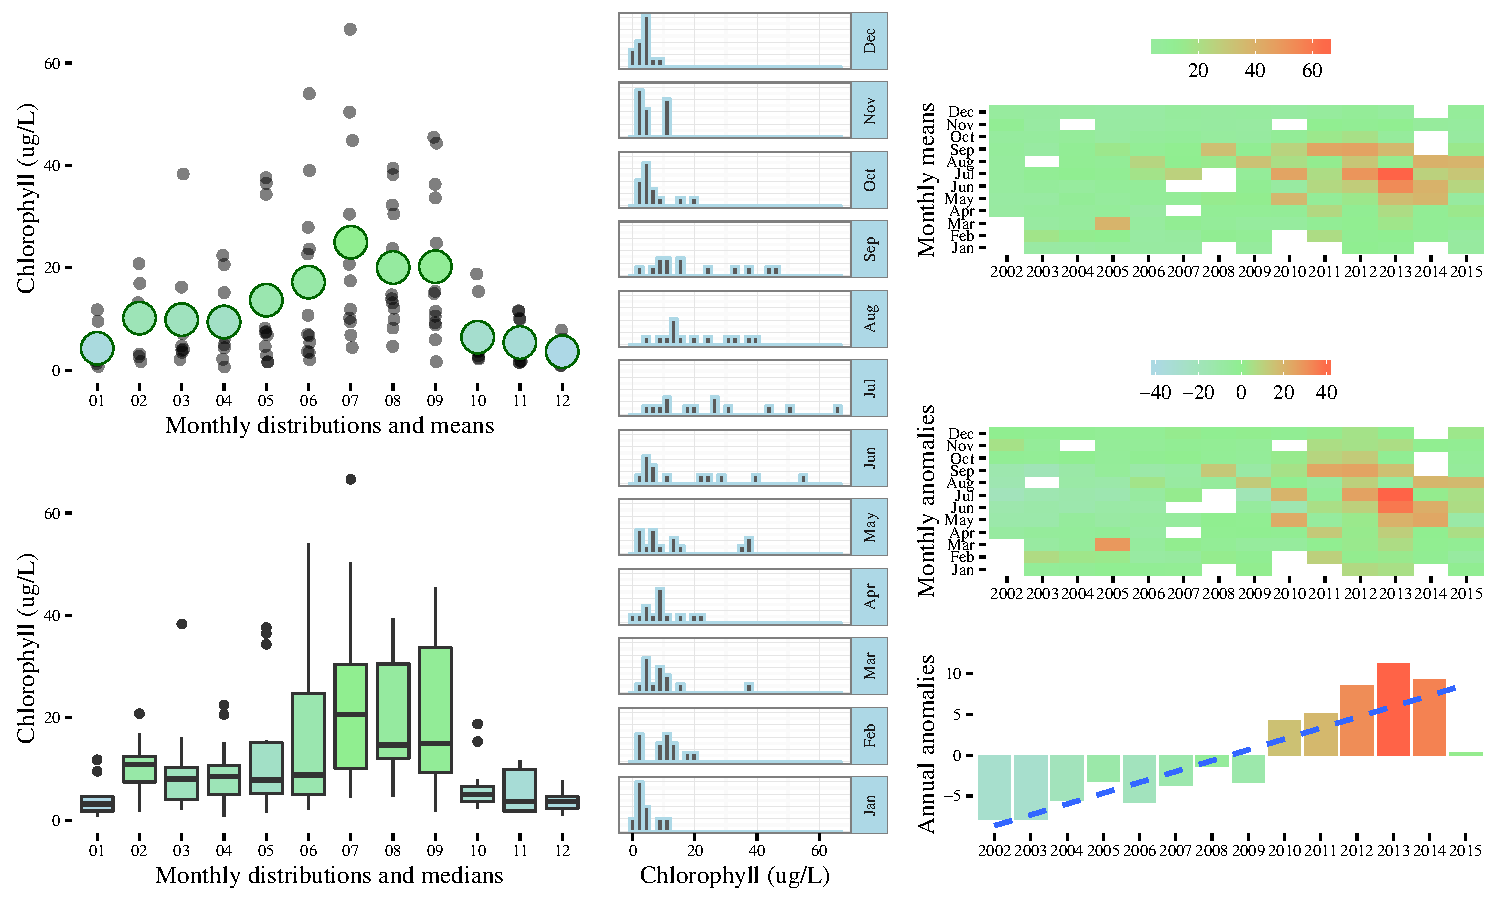
\includegraphics[width=0.8\textwidth]{imgs/unnamed-chunk-9-1} 

}



\end{knitrout}
\end{frame}

%%%%%%
\begin{frame}[fragile, t]{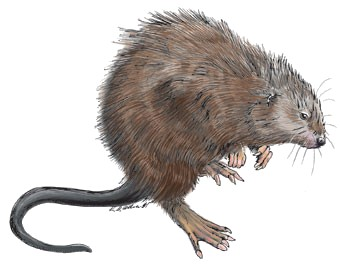
\includegraphics[width = 0.05\textwidth]{imgs/swmprat.png} Using \texttt{kendallTrendTest} with NERRS data}
Option 1: aggregate by years
\begin{knitrout}\scriptsize
\definecolor{shadecolor}{rgb}{0.969, 0.969, 0.969}\color{fgcolor}\begin{kframe}
\begin{alltt}
\hlcom{# get annual averages}
\hlstd{nutyr} \hlkwb{<-} \hlkwd{aggreswmp}\hlstd{(nut,} \hlkwc{by} \hlstd{=} \hlstr{'years'}\hlstd{)}

\hlcom{# convert datetimestamp to numeric for year}
\hlstd{nutyr}\hlopt{$}\hlstd{yr} \hlkwb{<-} \hlkwd{year}\hlstd{(nutyr}\hlopt{$}\hlstd{datetimestamp)}

\hlcom{# run test}
\hlstd{ests_k2} \hlkwb{<-} \hlkwd{kendallTrendTest}\hlstd{(chla_n} \hlopt{~} \hlstd{yr, nutyr)}
\hlstd{ests_k2}\hlopt{$}\hlstd{estimate}
\end{alltt}
\begin{verbatim}
##           tau         slope     intercept 
##     0.7582418     1.3938194 -2789.7357522
\end{verbatim}
\begin{alltt}
\hlstd{ests_k2}\hlopt{$}\hlstd{p.value}
\end{alltt}
\begin{verbatim}
##            z 
## 0.0001971407
\end{verbatim}
\end{kframe}
\end{knitrout}
\end{frame}

%%%%%%
\begin{frame}[fragile, t]{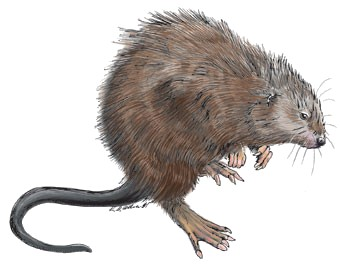
\includegraphics[width = 0.05\textwidth]{imgs/swmprat.png} Using \texttt{kendallSeasonalTrendTest} with NERRS data}
Option 2: use \texttt{kendallSeasonalTrendTest}
\begin{knitrout}\scriptsize
\definecolor{shadecolor}{rgb}{0.969, 0.969, 0.969}\color{fgcolor}\begin{kframe}
\begin{alltt}
\hlcom{# some additional prep for season and year columns}
\hlstd{nut}\hlopt{$}\hlstd{season} \hlkwb{<-} \hlkwd{month}\hlstd{(nut}\hlopt{$}\hlstd{datetimestamp)}
\hlstd{nut}\hlopt{$}\hlstd{yr} \hlkwb{<-} \hlkwd{year}\hlstd{(nut}\hlopt{$}\hlstd{datetimestamp)}

\hlcom{# run test}
\hlstd{ests_sk} \hlkwb{<-} \hlkwd{kendallSeasonalTrendTest}\hlstd{(chla_n} \hlopt{~} \hlstd{season} \hlopt{+} \hlstd{yr,} \hlkwc{data} \hlstd{= nut)}
\hlstd{ests_sk}\hlopt{$}\hlstd{estimate}
\end{alltt}
\begin{verbatim}
##          tau        slope    intercept 
##     0.423886     0.907000 -1354.312500
\end{verbatim}
\begin{alltt}
\hlstd{ests_sk}\hlopt{$}\hlstd{p.value}
\end{alltt}
\begin{verbatim}
## Chi-Square (Het)        z (Trend) 
##     7.346318e-02     9.868358e-17
\end{verbatim}
\end{kframe}
\end{knitrout}
\end{frame}

\section{Summary}

%%%%%%
\begin{frame}[t, fragile, shrink]{Summary}{}
\underline{\Bigtxt{Kendall}}
\begin{knitrout}\scriptsize
\definecolor{shadecolor}{rgb}{0.969, 0.969, 0.969}\color{fgcolor}\begin{kframe}
\begin{verbatim}
##       tau     slope intercept 
##     0.315     0.887 -1772.618
##       z 
## 2.1e-11
##   LCL   UCL 
## 0.606 1.185
\end{verbatim}
\end{kframe}
\end{knitrout}
\underline{\Bigtxt{Kendall by yr}}
\begin{knitrout}\scriptsize
\definecolor{shadecolor}{rgb}{0.969, 0.969, 0.969}\color{fgcolor}\begin{kframe}
\begin{verbatim}
##       tau     slope intercept 
##     0.758     1.394 -2789.736
##        z 
## 0.000197
##   LCL   UCL 
## 0.709 2.014
\end{verbatim}
\end{kframe}
\end{knitrout}
\underline{\Bigtxt{Seasonal Kendall}}
\begin{knitrout}\scriptsize
\definecolor{shadecolor}{rgb}{0.969, 0.969, 0.969}\color{fgcolor}\begin{kframe}
\begin{verbatim}
##       tau     slope intercept 
##     0.424     0.907 -1354.312
## Chi-Square (Het)        z (Trend) 
##         7.35e-02         9.87e-17
##   LCL   UCL 
## 0.667 1.209
\end{verbatim}
\end{kframe}
\end{knitrout}
\end{frame}

%%%%%%
\begin{frame}{Summary}{}
\onslide<1->
Final comments: \\~\\
\begin{itemize}
\item<1-> If you expect cyclical variation - aggregate to remove or use Seasonal Kendall \\~\\
\item<2-> Seasonal Kendall requires more work but has more power \\~\\
\item<3-> All of the above methods only detect a monotonic trend, do not account for other variables \\~\\
\item<4-> You can pick your time interval or use an alternative approach (e.g., WRTDS)
\end{itemize}
\end{frame}

%%%%%%
\begin{frame}
\vspace{0.3in}
\centerline{
\begin{tikzpicture}
  \node[drop shadow={shadow xshift=0ex,shadow yshift=0ex},fill=white,draw] at (0,0) {
\includegraphics[width=0.9\textwidth]{imgs/workshop2016logo.png}};
\end{tikzpicture}}
\vspace{0.5in}
\centerline{Up next... nothing!}
\vspace{0.5in}
\Large
\centerline{\Bigtxt{Questions??}}
\end{frame}

%%%%%%
\section{References}
\begin{frame}[t]{\textbf{References}}
\tiny
\setbeamertemplate{bibliography item}{}
\bibliographystyle{apalike_mine}
\bibliography{refs}
\end{frame}

\end{document}
